\begin{figure*}[!htbp]
\centering
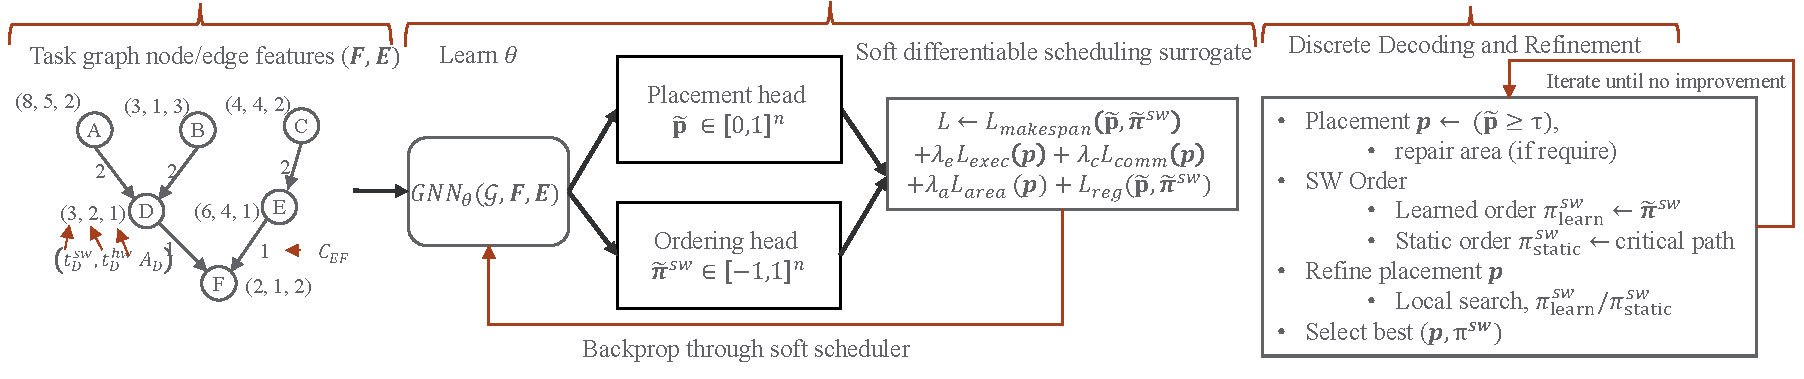
\includegraphics[width=1.0\linewidth]{Figures/methods/GNN_placement_order.pdf}
\caption{\sid{placeholder} Overview of \diffgnn for joint HW/SW partitioning and scheduling. A GNN encoder maps task graph features to the relaxed placement vector $\tilde{\vp}$ and relaxed software-priority vector $\tilde{\vpi}^{sw}$. A differentiable scheduling surrogate enables end-to-end optimization of makespan under constraints. At inference, solutions are discretized, repaired for feasibility, optionally refined, and evaluated using both the learned software order and a heuristic static-priority order; the better schedule is retained.}
\label{fig:diff_gnn_architecture}
\end{figure*}

\section{Proposed Method: \diffgnn}
\label{sec:method}

Building on the relaxed formulation in Section~\ref{sec:preliminaries}, we propose \diffgnn, a differentiable graph neural framework for jointly optimizing HW/SW partitioning and scheduling. Rather than directly searching over the discrete placement vector $\vp \in \{0,1\}^n$ and software order $\pi^{sw}$, \diffgnn learns a relaxed hardware-assignment vector $\tilde{\vp}\in[0,1]^n$ together with a relaxed software-priority vector $\tilde{\vpi}^{sw}\in[-1,1]^n$, and optimizes the relaxed objective in Equation~\eqref{eq:relaxed_obj} end-to-end using gradient-based learning.

Figure~\ref{fig:diff_gnn_architecture} illustrates the overall pipeline. Given a task graph $\gG(\gV,\gE)$, we first construct node and edge features, and a GNN encoder computes node embeddings that are then consumed by two prediction heads: (i) a \emph{placement head} that predicts relaxed hardware-assignment probabilities, and (ii) an \emph{ordering head} that predicts relaxed software priorities. These outputs are passed to an order-aware differentiable scheduler that approximates the makespan while accounting for both precedence constraints and software serialization. During inference, the relaxed solution is discretized, repaired if necessary to satisfy the area constraint, optionally refined, and finally evaluated using a discrete scheduler under two candidate software orders: the learned order induced by $\tilde{\vpi}^{sw}$ and a heuristic static-priority order. The better schedule is selected as the final output.


\subsection{Input Feature Preparation}

\paragraph{\textbf{Node features.}}
Each node $i \in \gV$ is associated with a feature vector capturing execution cost, resource usage, and structural properties:
\begin{equation}
\vf_i^{\mathrm{raw}} =
\left[
t_i^{sw},\;
t_i^{hw},\;
A_i,\;
d_i,\;
\frac{t_i^{hw}}{t_i^{sw}+\epsilon},\;
t_i^{sw}-t_i^{hw},\;
\frac{t_i^{sw}-t_i^{hw}}{\max(A_i,\epsilon)}
\right]
\in \mathbb{R}^7.
\end{equation}

Stacking all node features yields
\begin{equation}
\mF^{\mathrm{raw}} =
\begin{bmatrix}
(\vf_1^{\mathrm{raw}})^\top\\
\vdots\\
(\vf_n^{\mathrm{raw}})^\top
\end{bmatrix}
\in \mathbb{R}^{n\times 7}.
\end{equation}

We normalize features across nodes using column-wise z-score normalization:
\begin{equation}
\tilde{\mF} = \mathrm{Norm}(\mF^{\mathrm{raw}}).
\end{equation}

To incorporate the global hardware-area constraint, we append a constant feature:
\begin{equation}
\mF=
\begin{bmatrix}
\tilde{\mF} & \rho_A \mathbf{1}
\end{bmatrix}
\in\mathbb{R}^{n\times 8},
\end{equation}
where $\mathbf{1}\in\mathbb{R}^n$ is the all-ones vector.

\paragraph{\textbf{Edge features.}}
For each directed edge $(j,i)\in\gE$, we define an edge feature vector:
\begin{equation}
\ve_{ji}^{\mathrm{raw}} =
\left[
C_{ji},\;
|g_j-g_i|,\;
|ga_j-ga_i|
\right]
\in \mathbb{R}_{\ge 0}^3.
\end{equation}

Stacking all edges yields
\begin{equation}
\mE^{\mathrm{raw}} \in \mathbb{R}^{|\gE|\times 3}.
\end{equation}

We normalize edge features using column-wise max scaling:
\begin{equation}
\mE = \mathrm{Norm}_\infty(\mE^{\mathrm{raw}}),
\end{equation}
where $\mathrm{Norm}_\infty(\cdot)$ denotes feature-wise normalization by the maximum value.

\subsection{GNN Module}

\paragraph{\textbf{Message passing.}}
Let $\vh_i^{(0)}=\mF_{i,:}$ denote the initial node embedding. We use a message-passing GNN with $L$ layers:
\begin{equation}
\vh_i^{(\ell+1)}=
\phi^{(\ell)}\!\left(
\vh_i^{(\ell)},
\operatorname*{AGG}_{j:(j,i)\in\gE}
\psi^{(\ell)}\!\left(
\vh_i^{(\ell)},\;
\vh_j^{(\ell)},\;
\ve_{ji}
\right)
\right),
\end{equation}
for $\ell=0,\dots,L-1$, where $\phi^{(\ell)}$ and $\psi^{(\ell)}$ are learnable functions and $\operatorname*{AGG}$ is a permutation-invariant aggregation operator.

As a concrete instantiation, we use weighted mean aggregation:
\begin{align*}
\operatorname*{AGG}_{j:(j,i)\in\gE}
\psi^{(\ell)}\!\left(
\vh_i^{(\ell)},\;
\vh_j^{(\ell)},\;
\ve_{ji}
\right)
&=\frac{1}{\alpha}\sum_{j\in\gN(i)}\alpha_{\phi}(j,i)\,\mathbf{W}^{(\ell)}\vh_j^{(\ell)},\\
\alpha &= \sum_{j\in\gN(i)} \alpha_{\phi}(j,i)+\epsilon,
\end{align*}
where $\gN(i)$ denotes the set of incoming neighbors of node $i$, $\mathbf{W}^{(\ell)}$ is a learnable linear transformation, and $\alpha_{\phi}(j,i)\ge 0$ is a learnable edge weight derived from $\ve_{ji}$. We compute
\begin{equation}
\alpha_{\phi}(j,i)=\sigma\!\left(f_{\phi}(\ve_{ji})\right),
\end{equation}
where $f_{\phi}$ is an MLP and $\sigma(\cdot)$ is the sigmoid function.

\paragraph{\textbf{Placement head.}}
From the final embedding $\vh_i^{(L)}$, we predict relaxed hardware-assignment probabilities:
\begin{equation}
\tilde{p}_i = \sigma\!\left(\mathrm{MLP}_{\mathrm{place}}(\vh_i^{(L)})\right),
\end{equation}
where $\sigma(\cdot)$ denotes the sigmoid function, ensuring $\tilde{p}_i\in(0,1)$. Stacking all node-wise predictions gives
\begin{equation}
\tilde{\vp} = [\tilde{p}_1,\dots,\tilde{p}_n]^\top .
\end{equation}

\paragraph{\textbf{Ordering head.}}
To model software execution order, we compute bounded relaxed software-priority values:
\begin{equation}
\tilde{\pi}_i^{sw} = \tanh\!\left(\mathrm{MLP}_{\mathrm{order}}(\vh_i^{(L)})\right),
\end{equation}
so that $\tilde{\pi}_i^{sw}\in(-1,1)$. Stacking them yields
\begin{equation}
\tilde{\vpi}^{sw} = [\tilde{\pi}_1^{sw},\dots,\tilde{\pi}_n^{sw}]^\top \in \mathbb{R}^n.
\end{equation}


\subsection{Differentiable Soft Scheduler}

We now instantiate the relaxed makespan term $\widetilde{M}(\tilde{\vp},\tilde{\vpi}^{sw})$ from Section~\ref{sec:preliminaries}. The scheduler takes as input the relaxed placement vector $\tilde{\vp}$ and the relaxed software-priority vector $\tilde{\vpi}^{sw}$, and produces approximate start and finish times for all tasks.

The most important intermediate quantity is the effective software-order matrix $R^{sw}$. Figure~\ref{fig:soft_scheduler_walkthrough} illustrates its construction on a 6-node example. Read the figure from left to right:
\[
\tilde{\vpi}^{sw}
\;\rightarrow\;
\mP^{sw}
\;\rightarrow\;
\tilde{\vr}
\;\rightarrow\;
\mB^{sw}
\;\rightarrow\;
\mR^{sw}
\;\rightarrow\;
\widetilde{M}(\tilde{\vp},\tilde{\vpi}^{sw}).
\]

\begin{figure*}[t]
\centering
\setlength{\tabcolsep}{2.2pt}
\renewcommand{\arraystretch}{1.0}
\begin{adjustbox}{width=\textwidth,center}
\begin{tikzpicture}[
    >=Latex,
    font=\scriptsize,
    box/.style={draw=black!55, rounded corners=1pt, fill=gray!5, inner sep=2.2pt, align=center},
    arr/.style={-{Latex[length=1.8mm]}, very thick, draw=orange!85!black}
]

% =========================================================
% 1) GRAPH + INPUTS
% =========================================================
\node[anchor=north west] (graphbox) at (0,0) {%
\begin{minipage}{0.20\textwidth}
\centering
\begin{tikzpicture}[scale=0.68, every node/.style={font=\scriptsize}]
\node[circle,draw,fill=orange!85!yellow,inner sep=1.6pt,label=above:{A $(8,5,2)$}] (A) at (0,1.8) {};
\node[circle,draw,fill=orange!85!yellow,inner sep=1.6pt,label=above:{B $(3,1,3)$}] (B) at (1.9,1.8) {};
\node[circle,draw,fill=orange!85!yellow,inner sep=1.6pt,label=above:{C $(4,4,2)$}] (C) at (3.8,1.8) {};
\node[circle,draw,fill=black!90,inner sep=1.6pt,label=left:{D $(3,2,1)$}] (D) at (0.95,0.7) {};
\node[circle,draw,fill=black!90,inner sep=1.6pt,label=right:{E $(6,4,1)$}] (E) at (2.85,0.7) {};
\node[circle,draw,fill=black!90,inner sep=1.6pt,label=below:{F $(2,1,2)$}] (F) at (1.90,-0.35) {};
\draw[->,thin] (A)-- node[left] {\scriptsize 2} (D);
\draw[->,thin] (B)-- node[left] {\scriptsize 2} (D);
\draw[->,thin] (C)-- node[right] {\scriptsize 2} (E);
\draw[->,thin] (D)-- node[below] {\scriptsize 0} (F);
\draw[->,thin] (E)-- node[below] {\scriptsize 0} (F);
\end{tikzpicture}

\vspace{0.8mm}
$\tilde{\vp}=[0.05,0.05,0.05,0.95,0.95,0.95]^\top$

$\tilde{\vpi}^{sw}=[0.00,-1.00,1.00,-0.50,-0.75,-0.25]^\top$

Induced SW order: $C \prec A \prec B$
\end{minipage}
};

% =========================================================
% 2) ORDER VECTOR
% =========================================================
\node[box, anchor=north west] (qtab) at (4.25,0) {%
\begin{tabular}{c|c}
Task & $\tilde{\pi}^{sw}$\\\hline
A & \textcolor{red}{0.00}\\
B & \textcolor{red}{-1.00}\\
C & \textcolor{red}{1.00}\\
D & -0.50\\
E & -0.75\\
F & -0.25
\end{tabular}
};

% =========================================================
% 3) SINKHORN MATRIX
% =========================================================
\node[box, anchor=north west] (pmat) at (6.15,0) {%
\begin{tabular}{c|cccccc}
$u_a$ & A & B & C & D & E & F\\\hline
1.0  & 0.181 & 0.002 & \textcolor{red}{0.695} & 0.029 & 0.008 & 0.084\\
0.6  & \textcolor{red}{0.332} & 0.015 & 0.257 & 0.120 & 0.047 & 0.229\\
0.2  & 0.271 & 0.060 & 0.043 & 0.218 & 0.128 & 0.280\\
-0.2 & 0.143 & 0.155 & 0.005 & 0.255 & 0.224 & 0.219\\
-0.6 & 0.056 & 0.302 & 0.000 & 0.223 & 0.291 & 0.128\\
-1.0 & 0.017 & \textcolor{red}{0.467} & 0.000 & 0.155 & 0.302 & 0.060
\end{tabular}
};

\node[font=\scriptsize] at ($(pmat.south)+(0,-0.28)$)
{$L_{ai}=-(\tilde{\pi}^{sw}_i-u_a)^2/\tau_o,\quad \mP^{sw}=\mathrm{Sinkhorn}(L)$};

% =========================================================
% 4) RANK TABLE
% =========================================================
\node[box, anchor=north west] (rtab) at (11.10,0) {%
\begin{tabular}{c|c}
Task & $\tilde r_i$\\\hline
A & \textcolor{red}{1.613}\\
B & \textcolor{red}{4.141}\\
C & \textcolor{red}{0.357}\\
D & 2.986\\
E & 3.649\\
F & 2.258
\end{tabular}
};

\node[font=\scriptsize] at ($(rtab.south)+(0,-0.28)$)
{$\tilde r_i=\sum_{a=0}^{n-1} a\,\mP^{sw}_{ai}$};

% =========================================================
% 5) COMBINED GATE + BEFORE BOX
% =========================================================
\node[box, anchor=north west] (gbbox) at (13.00,0) {%
\begin{minipage}{0.23\textwidth}
\centering
$\displaystyle
G^{sw}=(1-\tilde{\vp})(1-\tilde{\vp})^\top=
\begin{bmatrix}
0.903\,\mathbf{1}_{3\times3} & 0.048\,\mathbf{1}_{3\times3}\\
0.048\,\mathbf{1}_{3\times3} & 0.003\,\mathbf{1}_{3\times3}
\end{bmatrix}
$

\vspace{0.8mm}
\begin{tabular}{c|cccccc}
 & A & B & C & D & E & F\\\hline
A & 0     & 0.999 & 0.027 & 0.981 & 0.997 & 0.863\\
B & 0.001 & 0     & 0     & 0.036 & 0.197 & 0.005\\
C & \textcolor{red}{0.973} & \textcolor{red}{1.000} & 0 & 0.999 & 1.000 & 0.996\\
D & 0.019 & 0.964 & 0.001 & 0 & 0.869 & 0.111\\
E & 0.003 & 0.803 & 0 & 0.131 & 0 & 0.018\\
F & 0.137 & 0.995 & 0.004 & 0.889 & 0.982 & 0
\end{tabular}

\vspace{0.6mm}
$\displaystyle B^{sw}_{ji}=\sigma\!\left(\frac{\tilde r_i-\tilde r_j}{\tau_r}\right)$
\end{minipage}
};

% =========================================================
% 6) FINAL RESOURCE MATRIX
% =========================================================
\node[box, anchor=north west] (rmat) at (18.00,0) {%
\begin{tabular}{c|cccccc}
 & A & B & C & D & E & F\\\hline
A & 0     & 0.902 & \textcolor{red}{0.024} & 0.047 & 0.047 & 0.041\\
B & 0.001 & 0     & 0     & 0.002 & 0.009 & 0\\
C & \textcolor{red}{0.878} & \textcolor{red}{0.902} & 0 & 0.047 & 0.047 & 0.047\\
D & 0.001 & 0.046 & 0 & 0 & 0.002 & 0\\
E & 0 & 0.038 & 0 & 0 & 0 & 0\\
F & 0.006 & 0.047 & 0 & 0.002 & 0.002 & 0
\end{tabular}
};

\node[font=\scriptsize] at ($(rmat.south)+(0,-0.28)$)
{$R^{sw}=B^{sw}\odot G^{sw}$};

\node[font=\scriptsize] at ($(rmat.south)+(0,-0.68)$)
{Key entries: $R^{sw}_{CA}=0.878,\;R^{sw}_{CB}=0.902,\;R^{sw}_{AB}=0.902$};

% =========================================================
% 7) MAKESPAN BOX
% =========================================================
\node[anchor=north west] (mspan) at (22.65,0) {%
\begin{minipage}{0.27\textwidth}
\centering
\textbf{From $R^{sw}$ to relaxed makespan}

\vspace{0.8mm}
Using the induced order $C \prec A \prec B$:
\[
\tilde f_C=4.00,\quad \tilde f_A=11.85,\quad \tilde f_B=14.75
\]
\[
\tilde s_D=16.55,\ \tilde f_D=18.60,\qquad
\tilde s_E=5.80,\ \tilde f_E=9.90
\]
\[
\tilde s_F=18.60,\qquad \tilde f_F=19.65
\]
\[
\widetilde{M}(\tilde{\vp},\tilde{\vpi}^{sw})
=
\mathrm{SMax}_{\beta}\!\big(\{\tilde f_i:i\in\Sink(\gG)\}\big)
\approx 19.65
\]

Alternative order $A \prec B \prec C$:
\[
\tilde f_F\approx 21.70
\]
Hence the learned ordering reduces the relaxed makespan.
\end{minipage}
};

% =========================================================
% ARROWS
% =========================================================
\draw[arr] (graphbox.east) -- (qtab.west);
\draw[arr] (qtab.east) -- (pmat.west);
\draw[arr] (pmat.east) -- (rtab.west);
\draw[arr] (rtab.east) -- (gbbox.west);
\draw[arr] (gbbox.east) -- (rmat.west);
\draw[arr] (rmat.east) -- (mspan.west);

\end{tikzpicture}
\end{adjustbox}
\caption{Numerical walk-through of the soft scheduler on a 6-node example. The example graph and relaxed inputs are followed by the ordering vector, Sinkhorn soft permutation matrix, expected ranks, gated rank-based precedence structure, effective software-order matrix $R^{sw}$, and the resulting relaxed makespan computation. The highlighted entries show that the example strongly favors the software order $C \prec A \prec B$.}
\label{fig:soft_scheduler_walkthrough}
\end{figure*}
First, the ordering head predicts relaxed software priorities $\tilde{\vpi}^{sw}$. These values are converted into a soft permutation matrix $\mP^{sw}$ using Sinkhorn normalization; $\mP^{sw}$ is then mapped to expected ranks $\tilde r_i$; the ranks are converted into a pairwise before matrix $\mB^{sw}$; and finally $\mB^{sw}$ is gated by the software co-assignment matrix so that ordering affects only tasks that are likely mapped to software. The same figure then shows how the resulting order propagates to the relaxed start and finish times and, ultimately, to the relaxed makespan.

\paragraph{\textbf{From relaxed software priorities to the effective software-order matrix.}}
The ordering head outputs
\begin{equation}
\tilde{\vpi}^{sw}=[\tilde{\pi}_1^{sw},\ldots,\tilde{\pi}_n^{sw}]^\top.
\end{equation}
We first construct a score-to-position compatibility matrix
\begin{equation}
L_{ai}=-\frac{(\tilde{\pi}_i^{sw}-u_a)^2}{\tau_o},
\qquad
u_a=1-\frac{2a}{n-1},
\quad a=0,\ldots,n-1,
\end{equation}
where $\{u_a\}_{a=0}^{n-1}$ are evenly spaced position anchors and $\tau_o$ controls the sharpness of the relaxation. Applying Sinkhorn normalization gives
\begin{equation}
\mP^{sw}=\mathrm{Sinkhorn}(L)\in[0,1]^{n\times n},
\end{equation}
where $\mP^{sw}_{ai}$ is the soft probability that task $i$ occupies position $a$ in the software order.

Next we compute the expected rank of each task:
\begin{equation}
\tilde r_i=\sum_{a=0}^{n-1} a\,\mP^{sw}_{ai}.
\end{equation}
A smaller $\tilde r_i$ indicates that task $i$ is predicted to execute earlier on software. We then convert these ranks into pairwise precedence scores:
\begin{equation}
B^{sw}_{ji}
=
\sigma\!\left(\frac{\tilde r_i-\tilde r_j}{\tau_r}\right),
\qquad
B^{sw}_{ii}=0,
\end{equation}
so that $B^{sw}_{ji}$ is large when task $j$ is likely to execute before task $i$.

Since ordering matters only when both tasks are likely assigned to software, we gate the pairwise precedence by
\begin{equation}
G^{sw}=(1-\tilde{\vp})(1-\tilde{\vp})^\top,
\end{equation}
and define the effective software-order matrix
\begin{equation}
R^{sw}_{ji}=B^{sw}_{ji}(1-\tilde{p}_j)(1-\tilde{p}_i)
\;=\;
B^{sw}_{ji}G^{sw}_{ji}.
\end{equation}
Thus, $R^{sw}_{ji}$ is large only when task $j$ is likely to precede task $i$ \emph{and} both tasks are likely mapped to software. In the example of Figure~\ref{fig:soft_scheduler_walkthrough}, this gives large entries such as $R^{sw}_{CA}=0.878$, $R^{sw}_{CB}=0.902$, and $R^{sw}_{AB}=0.902$, which strongly favor the software order $C\prec A\prec B$.

\paragraph{\textbf{Relaxed execution and communication.}}
The relaxed execution time of node $i$ is
\begin{equation}
\tilde{t}_i(\tilde{\vp})=\tilde{p}_i t_i^{hw} + (1-\tilde{p}_i)t_i^{sw},
\end{equation}
and the relaxed communication delay on edge $(j,i)$ is
\begin{equation}
\tilde{c}_{ji}(\tilde{\vp})=|\tilde{p}_j-\tilde{p}_i|\,C_{ji}.
\end{equation}

\paragraph{\textbf{DAG readiness.}}
Let $\Pred(i)$ denote the set of predecessors of node $i$. The DAG-readiness term is
\begin{equation}
s_i^{dag}
=
\begin{cases}
0, & \Pred(i)=\emptyset,\\[4pt]
\mathrm{SMax}_{\beta}
\Big(
\{\, \tilde{f}_j + \tilde{c}_{ji}(\tilde{\vp}) \mid j \in \Pred(i)\,\}
\Big), & \text{otherwise},
\end{cases}
\end{equation}
where
\begin{equation}
\mathrm{SMax}_{\beta}(\{a_k\})=\frac{1}{\beta}\log\sum_k e^{\beta a_k}.
\end{equation}
Intuitively, $s_i^{dag}$ is the earliest soft time at which task $i$ becomes ready from the precedence perspective.

\paragraph{\textbf{Software readiness.}}
Because software tasks execute sequentially on a single CPU, task $i$ may also need to wait for software tasks predicted to execute before it. We model this using $R^{sw}$:
\begin{equation}
\phi_{sw}(\tilde{\pi}_j^{sw},\tilde{\pi}_i^{sw})
=
\alpha \log(R^{sw}_{ji}+\epsilon),
\end{equation}
and define the software-readiness term as
\begin{equation}
s_i^{sw}
=
\mathrm{SMax}_{\beta}
\Big(
\{\, \tilde{f}_j + \phi_{sw}(\tilde{\pi}_j^{sw},\tilde{\pi}_i^{sw}) \mid j \neq i\,\}
\Big).
\end{equation}
If $R^{sw}_{ji}$ is large, then task $j$ is likely to delay task $i$ on the software processor.

\paragraph{\textbf{Start and finish times.}}
The relaxed start time of node $i$ is obtained by combining DAG and software readiness:
\begin{equation}
\tilde{s}_i=\mathrm{SMax}_{\beta}\big(\{s_i^{dag},\,s_i^{sw}\}\big),
\end{equation}
and the corresponding relaxed finish time is
\begin{equation}
\tilde{f}_i=\tilde{s}_i+\tilde{t}_i(\tilde{\vp}).
\end{equation}

\paragraph{\textbf{Soft makespan.}}
Let $\Sink(\gG)$ denote the set of sink nodes in $\gG$. The relaxed makespan is
\begin{equation}
L_{\mathrm{soft\mbox{-}makespan}}(\tilde{\vp},\tilde{\vpi}^{sw})
=
\widetilde{M}(\tilde{\vp},\tilde{\vpi}^{sw})
=
\mathrm{SMax}_{\beta}\big(\{\, \tilde{f}_i \mid i \in \Sink(\gG)\,\}\big).
\end{equation}

Figure~\ref{fig:soft_scheduler_walkthrough} also shows why the induced order $C\prec A\prec B$ is useful in this example: it starts the $C\!\rightarrow\!E$ branch earlier, which reduces the final relaxed makespan. Appendix~\ref{app:illustration} provides the full numerical walk-through of the resulting start and finish times.

\subsection{Training Objective}

The base relaxed objective is given in Equation~\eqref{eq:relaxed_obj}. In practice, we augment it with auxiliary execution, communication, and regularization terms:
\begin{equation}
L
=
L_{\mathrm{makespan}}(\tilde{\vp},\tilde{\vpi}^{sw})
+
\lambda_e L_{\mathrm{exec}}(\tilde{\vp})
+
\lambda_c L_{\mathrm{comm}}(\tilde{\vp})
+
\lambda_a L_{\mathrm{area}}(\tilde{\vp})
+
L_{\mathrm{reg}}(\tilde{\vp},\tilde{\vpi}^{sw}).
\end{equation}

Here, $L_{\mathrm{makespan}}$ captures the differentiable scheduling objective, while $L_{\mathrm{exec}}$ and $L_{\mathrm{comm}}$ correspond to relaxed execution and communication costs, respectively.

\paragraph{\textbf{Execution and communication losses.}}
We directly treat the relaxed execution and communication terms as auxiliary losses:
\begin{equation}
L_{\mathrm{exec}}(\tilde{\vp}) = \sum_{i\in\gV}\tilde{t}_i(\tilde{\vp}),
\qquad
L_{\mathrm{comm}}(\tilde{\vp}) = \sum_{(j,i)\in\gE}\tilde{c}_{ji}(\tilde{\vp}).
\end{equation}

The execution and communication terms regularize the optimization by discouraging slow assignments and excessive cross-partition communication, thereby aiding makespan minimization.

\paragraph{\textbf{Area constraint.}}
To enforce the hardware budget during training, we replace the hard constraint with a differentiable hinge penalty:
\begin{equation}
L_{\mathrm{area}}(\tilde{\vp})
=
\left[
\max\!\left(
0,\sum_{i\in\gV}\tilde{p}_i A_i - A_{\max}
\right)
\right]^2.
\end{equation}

\paragraph{\textbf{Regularization.}}
We further introduce optional regularization to stabilize ordering predictions and encourage nearly discrete assignments:
\begin{equation}
L_{\mathrm{reg}}(\tilde{\vp},\tilde{\vpi}^{sw})
=
\lambda_b L_{\mathrm{binary}}(\tilde{\vp})
+
\lambda_p L_{\mathrm{perm}}(\mP^{sw}),
% +
% \lambda_u L_{\mathrm{usage}}(\tilde{\vp}),
\end{equation}
where
\begin{align}
L_{\mathrm{binary}}(\tilde{\vp})
&=
\frac{1}{n}\sum_{i=1}^n \tilde{p}_i(1-\tilde{p}_i),\\
L_{\mathrm{p}}(\mP^{sw})
&=
\|\mP^{sw}\mathbf{1}-\mathbf{1}\|_2^2
+
\|(\mP^{sw})^\top\mathbf{1}-\mathbf{1}\|_2^2,
\\
% L_{\mathrm{usage}}(\tilde{\vp})
% &=
% (\mu_p-\rho)^2,
% \qquad
% \mu_p=\frac{1}{n}\sum_{i=1}^n \tilde{p}_i.
\end{align}

The term $L_{\mathrm{binary}}$ pushes relaxed assignments toward discrete decisions. 
The term $L_{\mathrm{perm}}$ keeps the soft ordering matrix close to a valid permutation relaxation. 
% The term $L_{\mathrm{usage}}$ controls the overall hardware usage level by matching the mean assignment to a target ratio $\rho$.

\subsection{Discrete Inference: Decoding, Scheduling, and Refinement}
\label{subsec:inference}

The outputs of \diffgnn are converted into a feasible discrete solution through a discrete inference pipeline. This stage bridges the gap between the differentiable training surrogate and the final discrete scheduling objective.

\paragraph{\textbf{Decoding and candidate generation.}}
Given relaxed placement probabilities $\tilde{\vp}$, we generate a set of discrete candidate partitions by thresholding:
\begin{equation}
\hat{p}_i = \mathbb{I}[\tilde{p}_i \ge \tau_d], \qquad \tau_d \in \mathcal{T},
\end{equation}
where $\mathcal{T}$ is a set of decoding thresholds.

\paragraph{\textbf{Feasibility repair.}}
Decoded candidates may violate the hardware area constraint. For each candidate, we enforce feasibility:
\begin{equation}
\sum_{i \in \gV} \hat{p}_i A_i \le A_{\max}.
\end{equation}
When the area constraint is violated, we run a deterministic repair loop: we repeatedly move one task from hardware to software, choosing the hardware task with the lowest benefit-per-area priority. This continues until the hardware area is within budget, thereby guaranteeing feasibility. After that, if area remains, we optionally test software-to-hardware flips that still fit the remaining area and keep the move with the best makespan improvement; by default, only non-worsening moves are accepted.

\paragraph{\textbf{Software order computation.}}
For each feasible decoded placement $\hat{\vp}$, we construct two candidate software orders. The first is the \emph{learned order} $\pi_{\mathrm{learn}}^{sw}$, obtained by sorting the relaxed software-priority vector $\tilde{\vpi}^{sw}$. The second is the \emph{static-priority order} $\pi_{\mathrm{static}}^{sw}$, computed using the same critical-path priority rule as LSSP on the decoded placement $\hat{\vp}$. Specifically, let
\begin{equation}
t_i(\hat{\vp}) = \hat{p}_i t_i^{hw} + (1-\hat{p}_i)t_i^{sw},
\end{equation}
and
\begin{equation}
\mathrm{comm}_{ij}(\hat{\vp}) = \mathbb{I}[\hat{p}_i \neq \hat{p}_j]\, C_{ij}.
\end{equation}
The static priority of task $i$ is computed in reverse topological order as
\begin{equation}
\mathrm{Pri}(i)
=
t_i(\hat{\vp})
+
\max_{j\in \Succ(i)}
\left(
\mathrm{comm}_{ij}(\hat{\vp}) + \mathrm{Pri}(j)
\right),
\label{eq:lssp_priority}
\end{equation}
with $\mathrm{Pri}(i)=t_i(\hat{\vp})$ for sink tasks. Intuitively, $\mathrm{Pri}(i)$ estimates how critical task $i$ is to the final makespan. Figure~\ref{fig:staticpriorities} illustrates how these priorities are computed bottom-up. If there are multiple sink nodes, we add a dummy sink node and start the computation from there.

\begin{figure}[!htbp]
\centering
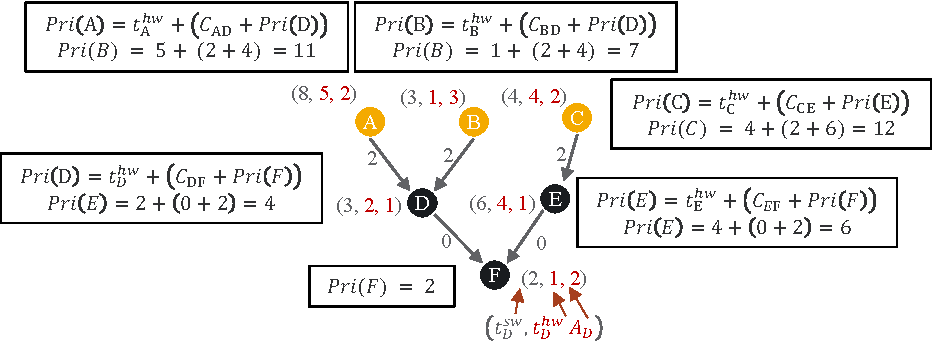
\includegraphics[width=1.0\linewidth]{Figures/methods/static_priorities.pdf}
\caption{\sid{placeholder} Example of bottom-up static-priority computation.}
\label{fig:staticpriorities}
\end{figure}

\paragraph{\textbf{Makespan computation.}}
Given a discrete placement $\hat{\vp}$, we run list scheduling twice, once with software order $\pi_{\mathrm{learn}}^{sw}$ and once with $\pi_{\mathrm{static}}^{sw}$. Let $k \in \{\mathrm{learn},\mathrm{static}\}$ denote the chosen software-order policy. At each scheduling event $t$, the next software task is selected from the ready software set
\begin{equation}
\mathcal{R}_{sw}(t)=\{i\mid \hat{p}_i=0,\ \Pred(i)\subseteq \mathcal{C}(t)\},
\qquad
i_t^{(k)}=\arg\max_{i\in\mathcal{R}_{sw}(t)} \pi_k^{sw}(i),
\end{equation}
with deterministic tie-breaking. Dependency readiness is
\begin{equation}
r_i^{(k)}=\max_{j\in\Pred(i)}\big(f_j^{(k)}+c_{ji}(\hat{\vp})\big),
\end{equation}
and start/finish times are
\begin{equation}
s_i^{(k)}=\max\!\big(r_i^{(k)},t_{i,\mathrm{avail}}^{(k)}\big),
\qquad
f_i^{(k)}=s_i^{(k)}+t_i(\hat{\vp}),
\end{equation}
where
\begin{equation}
t_{i,\mathrm{avail}}^{(k)}=
\begin{cases}
t_{SW,\mathrm{avail}}^{(k)}, & \hat{p}_i=0,\\
0, & \hat{p}_i=1,
\end{cases}
\end{equation}
and $t_{SW,\mathrm{avail}}^{(k)}$ is the current availability time of the single software lane, updated after each scheduled software task.

This yields two candidate makespans,
\begin{equation}
T^{\mathrm{learn}}=\max_i f_i^{(\mathrm{learn})},
\qquad
T^{\mathrm{static}}=\max_i f_i^{(\mathrm{static})}.
\end{equation}
For \diffgnn, we define the discrete evaluation score of placement $\hat{\vp}$ as
\begin{equation}
T^\star(\hat{\vp})
=
\min\!\big(T^{\mathrm{learn}},\,T^{\mathrm{static}}\big),
\label{eq:best_of_two_orders}
\end{equation}
and denote the corresponding selected software order by $\hat{\pi}^{sw}$.

\paragraph{\textbf{Optional local refinement.}}
Starting from the repaired placement, we optionally apply local search to explore local changes, such as flipping assignments of critical nodes. Each proposed move is evaluated using the discrete makespan score $T^\star(\hat{\vp})$, and a move is accepted only if it improves the current solution under this evaluation.

\paragraph{\textbf{Final selection.}}
Across all decoded candidates and their refined versions, we select the solution with the smallest final discrete makespan:
\begin{equation}
(\vp^\star,\pi^{sw,\star})
=
\arg\min_{(\hat{\vp},\hat{\pi}^{sw})\in\mathcal{C}}
M(\hat{\vp},\hat{\pi}^{sw}),
\end{equation}
where $\mathcal{C}$ denotes the set of all feasible decoded or refined placements together with their selected software orders. Equivalently, the final makespan reported for \diffgnn is the minimum value of $T^\star(\hat{\vp})$ over all candidates.

For competing algorithms, we use only the LS-based static-priority order, so that all baselines are evaluated under the same standard discrete scheduling rule.




\subsection{Pseudocode of \diffgnn}
Algorithms~\ref{alg:diffgnn_training} and~\ref{alg:diffgnn_inference} summarize the training and discrete inference procedures of \diffgnn.

\begin{algorithm}[!htbp]
\caption{Training of \diffgnn}
\label{alg:diffgnn_training}
\KwIn{Task graph $\gG=(\gV,\gE)$, epochs $T$, area budget $A_{\max}$}
\KwIn{Loss weights $\lambda_e,\lambda_c,\lambda_a,\lambda_b,\lambda_p$}
\KwIn{Temperatures $\tau_o,\tau_r$ and smooth-max parameter $\beta$}
Initialize model parameters $\theta$\;
Construct node and edge features $\mF,\mE$\;

\For{$t=1,\dots,T$}{
    Predict $\tilde{\vp},\tilde{\vpi}^{sw}\gets \mathrm{GNN}_{\theta}(\gG,\mF,\mE)$\;
    
    Build soft precedence from $\tilde{\vpi}^{sw}$ using Sinkhorn relaxation\;
    
    Compute relaxed execution/communication terms $\tilde{t}_i,\tilde{c}_{ji}$\;
    
    Run differentiable scheduler to obtain $\tilde{\vs},\tilde{\vf}$\;
    
    Compute $L_{\mathrm{makespan}},L_{\mathrm{exec}},L_{\mathrm{comm}},L_{\mathrm{area}},L_{\mathrm{reg}}$\;
    
    $L \gets L_{\mathrm{makespan}}
    + \lambda_e L_{\mathrm{exec}}
    + \lambda_c L_{\mathrm{comm}}
    + \lambda_a L_{\mathrm{area}}
    + L_{\mathrm{reg}}$\;
    
    Update $\theta$ via backpropagation\;
}
\end{algorithm}

\begin{algorithm}[!htbp]
\caption{Discrete Inference and Post-Processing}
\label{alg:diffgnn_inference}
\KwIn{Graph $\gG$, trained model, area budget $A_{\max}$, thresholds $\mathcal{T}$}
\KwOut{Best discrete placement $\vp^\star$, software order $\pi^{sw,\star}$, makespan $M^\star$}

Compute $\tilde{\vp},\tilde{\vpi}^{sw}$\;
Initialize $\vp^\star \gets \emptyset$, $\pi^{sw,\star}\gets\emptyset$, $M^\star \gets +\infty$\;

\For{$\tau_d \in \mathcal{T}$}{
    Decode $\hat{\vp}$ by thresholding:
    $\hat{p}_i \gets \mathbb{I}[\tilde{p}_i \ge \tau_d]$\;
    
    Repair $\hat{\vp}$ until $\sum_i \hat{p}_i A_i \le A_{\max}$\;
    
    Refine $\hat{\vp}$ using local search\tcp*[r]{optional}
    
    Compute learned software order $\pi_{\mathrm{learn}}^{sw}$ by sorting $\tilde{\vpi}^{sw}$\;
    Compute static-priority order $\pi_{\mathrm{static}}^{sw}$ on $\hat{\vp}$\;
    
    $T^{\mathrm{learn}} \gets M(\hat{\vp},\pi_{\mathrm{learn}}^{sw})$,
    $T^{\mathrm{static}} \gets M(\hat{\vp},\pi_{\mathrm{static}}^{sw})$\;
    
    $\hat{\pi}^{sw} \gets
    \arg\min_{\pi \in \{\pi_{\mathrm{learn}}^{sw},\,\pi_{\mathrm{static}}^{sw}\}}
    M(\hat{\vp},\pi)$\;
    
    $T^\star(\hat{\vp}) \gets
    \min\!\big(T^{\mathrm{learn}},\,T^{\mathrm{static}}\big)$\;
    
    \If{$T^\star(\hat{\vp}) < M^\star$}{
        $\vp^\star \gets \hat{\vp}$,\quad
        $\pi^{sw,\star} \gets \hat{\pi}^{sw}$,\quad
        $M^\star \gets T^\star(\hat{\vp})$\;
    }
}
\Return{$(\vp^\star,\pi^{sw,\star},M^\star)$}\;
\end{algorithm}




\subsection{Complexity Analysis}

\paragraph{\textbf{Training Complexity.}}
Let $n=|\gV|$, $m=|\gE|$, hidden size $d$, and $L$ GNN layers. The GNN and prediction heads incur a cost of $O\!\big(L(md + nd^2)\big) + O(nd)$. Applying Sinkhorn normalization to an $n \times n$ matrix costs $O(T_{\mathrm{sink}} n^2)$, where $T_{\mathrm{sink}}$ (typically $10$--$12$) is the number of normalization iterations, and computing rank-based pairwise precedence requires $O(n^2)$. The differentiable scheduler adds $O(m + n^2)$.

Thus, the total time complexity per forward pass is $T_{\text{total}} = O\!\big(L(md + nd^2) + m + T_{\mathrm{sink}} n^2 + n^2\big)$. The space complexity is $S_{\text{total}} = O(Lnd + m + n^2)$, where the $n^2$ term (dense ordering tensors) is the primary scalability bottleneck.


\paragraph{\textbf{Post-processing complexity.}}
For each decoded placement, post-processing requires computing the learned software order, the static-priority order, and evaluating discrete schedules under both. The overall cost per decoded placement is $O(m+n\log n)$. Thus, with $|\mathcal{T}|$ decoding thresholds and $R$ local-refinement evaluations, the total post-processing complexity is $O\!\big((|\mathcal{T}|+R)(m+n\log n)\big)$. In practice, this is much smaller than the training cost.

\paragraph{\textbf{Large-graph approximation.}}
For large-scale graphs, we improve scalability by skipping Sinkhorn normalization and directly using ordering logits for pairwise precedence, while restricting software ordering to the top-$k$ high-confidence nodes per task. This reduces pairwise interactions from $O(n^2)$ to $O(nk)$ with $k \ll n$, yielding $T_{\text{total}} = O\!\big(L(md+nd^2)+m+nk\big)$ and $S_{\text{total}} = O(Lnd+m+nk)$.